% Proposed main-body replacement. Preserve the existing
% \crossscaletablematerial definition separately for its appendix invocation.
\section{Experimental Design}
\label{sec:experiments}

We test verified memory as a separate intervention: first against fresh
reward optimization and direct alternatives, then alongside MaxRL, and
finally on harder tasks with matched solution counts. The Level-1 study
covers Qwen2.5-0.5B, Falcon3-1B, and Qwen2.5-3B across all five domains.
Level 2 repeats the four-method factorial at Qwen2.5-0.5B. A precheck
compares unmodified Dr.GRPO and GRPO before and after training; both lose
extra verified modes at every scale, although correctness and raw support
need not decline together (Appendix~\ref{app:pre-rl-regression}).

\phantomsection\label{sec:shared-protocol}
Training uses 384 prompts, rollout groups of 16, and eight passes.
At registered checkpoints, four fixed-seed draws of eight responses on
128 disjoint prompts measure co-primary \texttt{pass@8} and
\texttt{distinct@8}. Their difference counts extra correct modes and
remains coupled to correctness. Paired methods share initialization,
data, optimizer, decoding, and evaluation requests. Terminal comparisons
use five training seeds where complete; their unadjusted paired 95\%
intervals describe seed variation on the fixed benchmark. Partial
intersections report exact counts without intervals, and missing endpoints
are never imputed. Protocols, coverage, and complete trajectories are in
Appendices~\ref{app:reproducibility} and~\ref{app:supporting}.

\phantomsection\label{sec:retention-design}
\phantomsection\label{sec:factorial-design}
Dr.GRPO/ReplayDr.GRPO and MaxRL/ReplayMaxRL differ in the applied replay
derivative; controls execute the same bank and scoring code. GRPO, UCPO,
sparse RLEP-Dr, and fixed Semantic MaxEnt test alternative explanations.
UCPO and RLEP-Dr comparisons use only the 0.5B and 1B models.
\phantomsection\label{sec:levels-design}
Level 2 changes task structure while preserving validators, canonical keys,
and valid-mode-count histograms, so difficulty is not confounded with fewer
available solutions. Its prompt sets are disjoint from Level 1.

\section{Results}
\label{sec:results}

\subsection{Experiment 1: replay retains verified support across scale}
\label{sec:results-retention}

Replay improves both correctness and sampled support in every complete
Dr.GRPO model--domain block (Figure~\ref{fig:cross-scale-terminal-effects}).
Raw \texttt{distinct@8} increases in all 74 admissible paired seeds.
The remaining registered pair is excluded for conflicting source evaluations,
not its measured effect (Appendix~\ref{app:source-integrity}).

Countdown makes the distinction between success and alternatives concrete.
At Qwen2.5-0.5B, replay raises \texttt{pass@8} from $.480$ to $.672$ while
\texttt{distinct@8} rises from $.487$ to $1.637$. Because its keys identify
computation trees, the latter gain means more correct routes to the same
answer. Python and MathIR more often gain correctness without a comparable
extra-mode increase. The meaning of broader support therefore depends on
whether a domain's key denotes a route, behavior, or valid configuration.

\begin{figure}[!b]
  \centering
  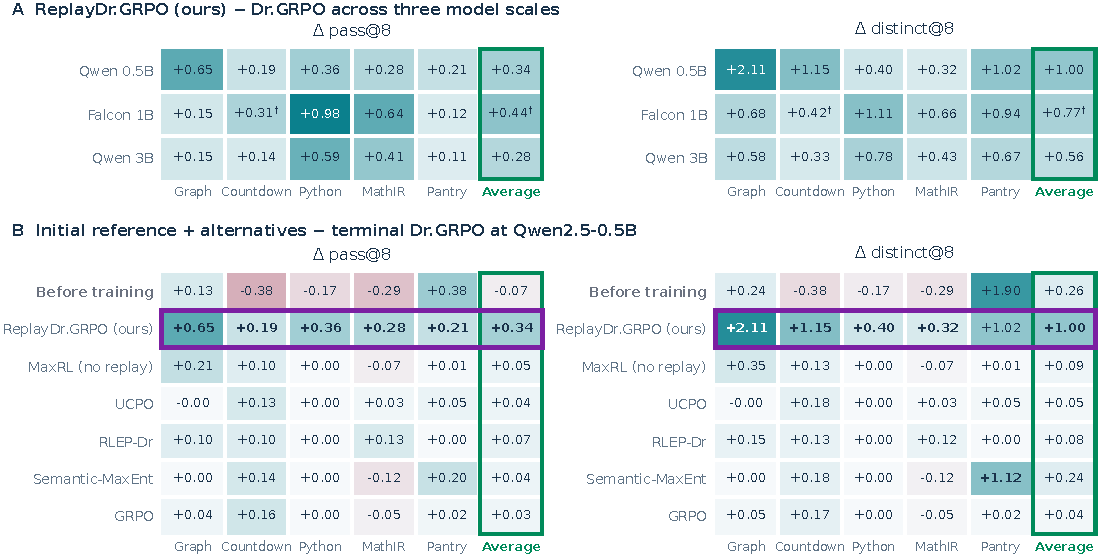
\includegraphics[width=\linewidth]{figures/experiment1_retention_comparator_matrix.pdf}
  \caption{\textbf{Replay improves correctness and verified support.}
  (A) ReplayDr.GRPO minus Dr.GRPO at all three scales.
  (B) Qwen2.5-0.5B alternatives minus Dr.GRPO. Columns have different units:
  probability points and expected verified-mode counts. Averages weight
  domains equally within seed. Daggers mark four admissible seeds in Falcon
  Countdown and its average; other cells use five. Only complete blocks
  receive unadjusted 95\% intervals. Purple identifies replay; bold marks
  the largest Panel-B means.}
  \label{fig:cross-scale-terminal-effects}
\end{figure}

The controls distinguish memory from generic improvement incentives.
ReplayDr.GRPO has the largest mean correctness gain among the direct
alternatives in every Qwen2.5-0.5B domain. A separate weighting ablation
keeps bank construction and update code fixed: uniform key weighting adds
$+.318$ extra modes over fresh-frequency weighting across those five
domains, while its correctness contrast remains inconclusive
(Appendix~\ref{app:frequency-replay-progress}). This supports a contribution
from key balancing, without a universal accuracy advantage.

\subsection{Experiment 2: memory remains useful beyond MaxRL}
\label{sec:results-maxrl}

Stronger fresh-rollout optimization does not remove the replay benefit.
At both scales with complete MaxRL pairs across all domains, replay raises
the cross-domain means of correctness and raw support
(Figure~\ref{fig:maxrl-factorial}). The same direction under Dr.GRPO and
MaxRL identifies an additional contribution from verified memory, rather
than dependence on one fresh objective. ``Complementary'' here means an
additional benefit; it does not assert a positive factorial interaction.

The larger model extends this comparison without completing the grid.
Qwen2.5-3B has complete Dr.GRPO pairs and domain-specific MaxRL populations;
its available-pair averages favor replay. Those descriptive summaries
cannot establish a complete five-seed factorial or a scaling law. Effects
also vary within completed scales: Falcon Graph's mean raw-support effect
is negative with an interval spanning zero. Full domain contrasts and both
training metrics remain in Appendix~\ref{app:maxrl-scale-extensions}.

\begin{figure}[!b]
  \centering
  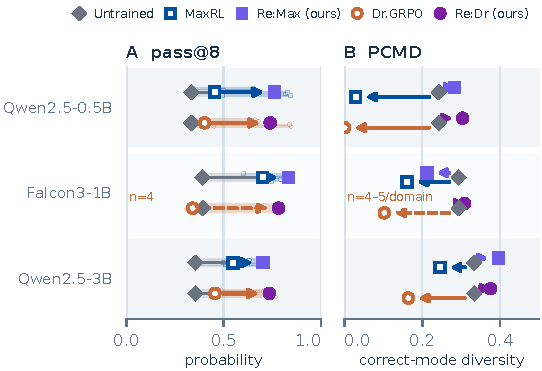
\includegraphics[width=\linewidth]{figures/e118_all_scale_factorial_progress.pdf}
  \caption{\textbf{Replay adds value under both fresh objectives at all three scales.}
  Rows compare MaxRL/ReplayMaxRL and Dr.GRPO/ReplayDr.GRPO on correctness
  and raw support. Diamonds are initial models; open/filled markers omit/apply
  replay. Complete tracks average domains within seed; faint paths show seeds.
  Falcon Dr.GRPO uses four common seeds. The dashed 3B MaxRL track weights
  domain means equally using Graph/Countdown/Python/MathIR/Pantry counts
  $5/3/5/3/1$, without a common seed trajectory or interval.}
  \label{fig:maxrl-factorial}
\end{figure}

\subsection{Experiment 3: replay transfers to harder matched tasks}
\label{sec:results-levels}

Replay raises both aggregate endpoints under both objectives on the four
complete Level-2 domains (Figure~\ref{fig:level2-admission}). Graph provides
the clearest evidence: replay increases correctness and extra modes after
either fresh objective. The other three domains have positive mean
correctness and raw-support effects with intervals including zero. The
transfer is therefore encouraging but uneven; improved support is not
established as the cause of improved correctness.

\begin{figure}[!t]
  \centering
  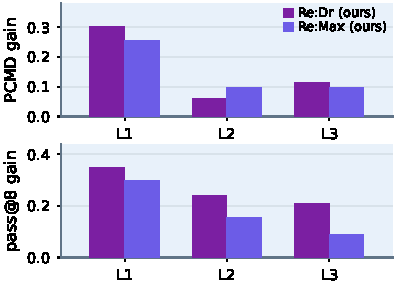
\includegraphics[width=.98\linewidth]{figures/modebench_level_admission.pdf}
  \caption{\textbf{Replay across difficulty levels at Qwen2.5-0.5B.}
  Open/filled markers identify Level 1/2. (A) Frozen-model success across
  all five domains. (B) Terminal means over Graph, Countdown, Python, and
  MathIR, weighted equally within five seeds shared by both levels and all
  four methods. Pantry's available arm counts are shown separately; it
  has no complete factorial and does not enter the average.}
  \label{fig:level2-admission}
\end{figure}

\section{Conclusion}
\label{sec:conclusion}
\label{sec:discussion}
\label{sec:limitations}

\mb{} distinguishes learning to succeed from retaining multiple verified
ways to succeed. Across objectives, scales, and the first matched increase
in difficulty, replay preserves more sampled alternatives while often
improving correctness. The paired interventions support memory's additional
value; they do not establish survival of every previously discovered mode
or downstream benefits from every added alternative.

\phantomsection\label{sec:hosted-concentration}
A separate inference-only evaluation of GPT-5.6 Sol and Claude Opus 5 also
finds concentrated outputs despite perfect Level-3 Graph correctness
(Appendix~\ref{app:hosted-comparison}). It provides context, not a matched
training comparison or evidence about the cause of concentration.

The guarantees remain conditional on idealized optimization and admitted
bank contents. Actual fixed-exemplar measurements retain a declining tail,
and finite banks cannot represent every available solution. Richer reasoning
tasks should test which alternatives survive and when preserving them helps
solve a later problem that an initially favored approach cannot.
